\documentclass{beamer}

\usepackage[beamer]{shortcut}

\usepackage{amsfonts}


\usepackage{array}
\usepackage{xcolor,colortbl}
\newcolumntype{a}{ >{\columncolor{blue}} c }

\usepackage{tikz}
\usepgflibrary{shapes.arrows}

\graphicspath{{./images/}}

\institute{INRIA Saclay}
\author{Thomas Moreau}
\title{
    A framework for bilevel optimization that enables stochastic and global variance reduction algorithms
}
\collaborators{M. Dagréou, P. Ablin, S. Vaiter and Z. Ramzi}

\setbeamertemplate{title page}[frame]
\def\extraLogo{}

\newcommand{\citeline}[1]{\textcolor{gray}{\small[{\color{linkcolor} #1}]}}
\newcommand{\blue}[1]{\textcolor{blue}{#1}}
\newcommand{\red}[1]{\textcolor{red}{#1}}


\def\biblio{
	\nobibliography{library}
	\def\biblio{}
}

\begin{document}

    \begin{frame}
        \titlepage
    	\biblio{}
    \end{frame}

    % 
    \frame{
        \frametitle{Learning a linear ML model}


        \textbf{Setup:}\\[1em]
        \begin{itemize}
            \item Binary classification task $(X_i, y_i)_{i=1}^N \in \mathbb R^p \times \{-1, 1\}$
            \item Linear model: predict $y$ from $X$ with $\text{sign}(\langle \theta, X\rangle)$.
        \end{itemize}

        {\centering
        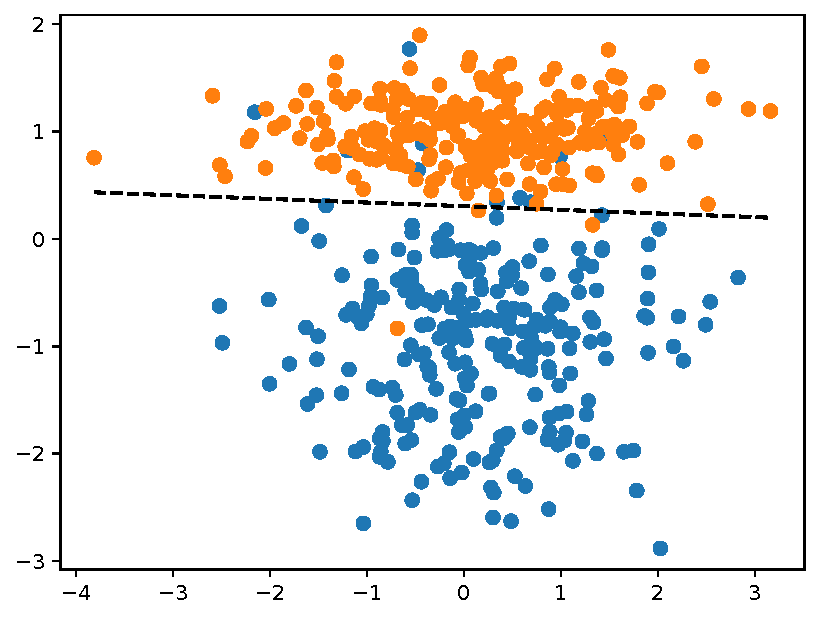
\includegraphics[width=.6\textwidth]{images/logreg_noreg}\\
        }

    }

    \frame{
        \frametitle{Learning a linear ML model}

        \textbf{Logistic loss:}\\[1em]

        \[
            G(\theta) = \frac1N \sum_{i=1}^N \log( 1 + e^{-y_i \langle \theta, X_i\rangle})
        \]


        \textbf{Training the model:}\\[1em]
        \[
            \theta^* = \argmin_\theta G(\theta)
        \]

    }

    \frame{
        \frametitle{Avoiding overfitting}

            Here, the second feature is uninformative,\\[2em]

            {\centering
            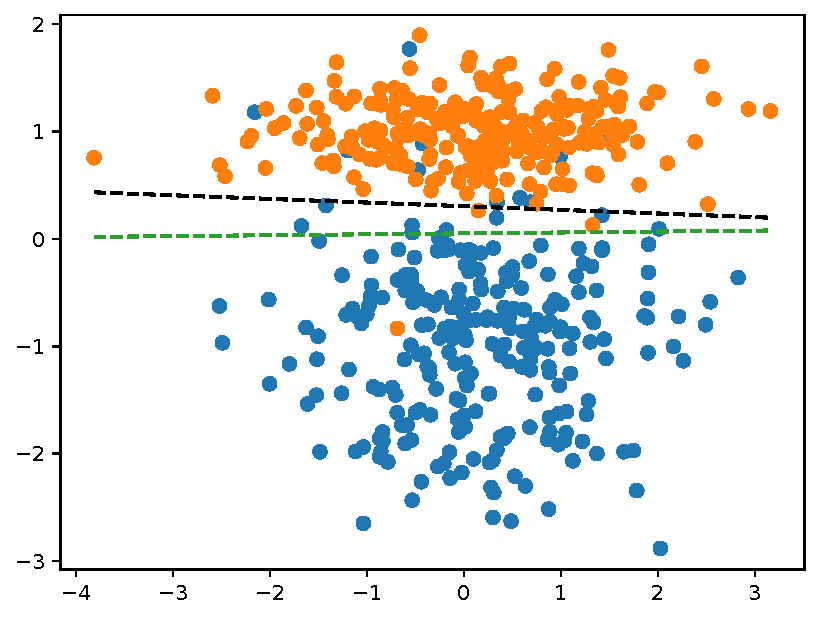
\includegraphics[width=.6\textwidth]{images/logreg_reg}\\
            }
    }
    \frame{
        \frametitle{Avoiding overfitting with a regularization}
        \textbf{\textcolor{blue!70}{Regularized} Logistic loss:}

        \[
            G(\theta, \lambda) = \frac1N \sum_{i=1}^N \log( 1 + e^{-y_i \langle \theta, X_i\rangle}) + \color{blue!70}\lambda\|\theta\|_2^2
        \]


        \textbf{Training the model:}\\[1em]
        \[
            \theta^*({\color{blue!70}\lambda}) = \argmin_\theta G(\theta,{\color{blue!70} \lambda})
        \]

        \pause
        \strongpoint{\bf \Large How to choose $\lambda$?}

    }

    \frame{
        \frametitle{Evaluating the generalization}

        We want to find $\lambda$ that ensure the best \emph{generalization} of $\theta^*(\lambda)$.\\[2em]

        \textbf{Validation loss:} use held out data $(X^{\it val}_i, y^{\it val}_i)_{i=1}^M$
        \[
            F(\theta) = \frac1M \sum_{i=1}^M \log( 1 + e^{-y^{\it val}_i \langle \theta, X_i^{\it val}\rangle})
        \]

        Independent estimate of the risk of the model.\\[1em]

        \pause
        \strongpoint{Find $\lambda$ that gives a model $\theta^*(\lambda)$ with a good validation loss.}
    }

    \frame{
        \frametitle{The Grid Search}

        \begin{itemize}\itemsep1.5em
            \item Select a grid of parameters $\{\lambda_1,\dots \lambda_K\}$.
            \item Train a model for each parameter $\lambda_k$: $\theta^*(\lambda_k)$.
            \item Evaluate the performance with the validation loss $F(\theta^*(\lambda_k))$.
            \item Keep the value $\lambda_k$ with the best performance.
        \end{itemize}

        \pause
        \vskip2em
        \textbf{Mathematical rewritting:}
        \[\begin{cases}
            \quad\min_{\lambda \in \{\lambda_1,\dots \lambda_K\}}
            F(\theta^*(\lambda))\\
            s.t.\quad \theta^*(\lambda) = \argmin_\theta G(\theta, \lambda)
        \end{cases}\]
    }

    \frame{
        \frametitle{The Grid Search with multiple hyperparameters}

        \textbf{Regularized Logistic loss:}

        \[
            G(\theta, \lambda) = \frac1N \sum_{i=1}^N \log( 1 + e^{-y_i \langle \theta, X_i\rangle}) + \alt<2->{\color{blue!70}\sum_{k=1}^p\lambda_k\theta_k^2}{\lambda\|\theta\|_2^2}
        \]

        \visible<2->{
            Grid search is inefficient as the grid increases exponentially with the number of parameters.
        }
        \vskip2em

        \visible<3>{
            \strongpoint{\bf\large Can we use first-order methods to minimize $h(\lambda) = F(\theta^*(\lambda))$?}
        }
    }

    \frame{
        \frametitle{Bi-level optimization}

        {\bf Bi-level problem:} Optimization problem with two levels\\[1em]
        \begin{align*}
            \min_\lambda ~& {\color{darkblue} h(\lambda)} = {\color{darkred}F(\lambda, \theta^*(\lambda))} \\[.5em]
                & s.t.\quad \theta^*(\lambda) = \argmin_\theta {\color{lightgreen}G(\lambda, \theta)}
        \end{align*}
        \begin{tikzpicture}[overlay]
            \draw[<-, thick, shorten >=8, darkblue] (4.1, 1.7) -- +(-1.5, -1.3) node[darkblue] {\emph{Value function}};
            \draw[<-, thick, shorten >=35,darkred] (7.3, 1.9) -- +(3, -.2) node {\emph{\color{darkred}Outer function}};
            \draw[<-, thick, shorten >=8, lightgreen] (8, .5) -- +(0, -.8) node {\emph{\color{lightgreen} Inner function/Problem}};
        \end{tikzpicture}

        \vskip3em
        {\bf Goal:}  Optimize the value function $h$ whose value depends on the result of another optimization problem.
    }
    \frame[t]{
        \frametitle{Bi-level optimization problems: Model selection}

        \vskip1em
        {\bf Selecting the best model:}\\[.5em]
        \begin{itemize}\itemsep.7em
            \item $G$ is the training loss and $\theta$ are the parameters of the model.
            \item Select the hyper-parameter $\lambda$ to get the best validation loss $F$.
        \end{itemize}
        \vskip1em
        \alt<2->{
            \alt<3>{
                {\bf Neural Architecture Search:} $\lambda$ parametrizes the architecture. \\

                {\centering
                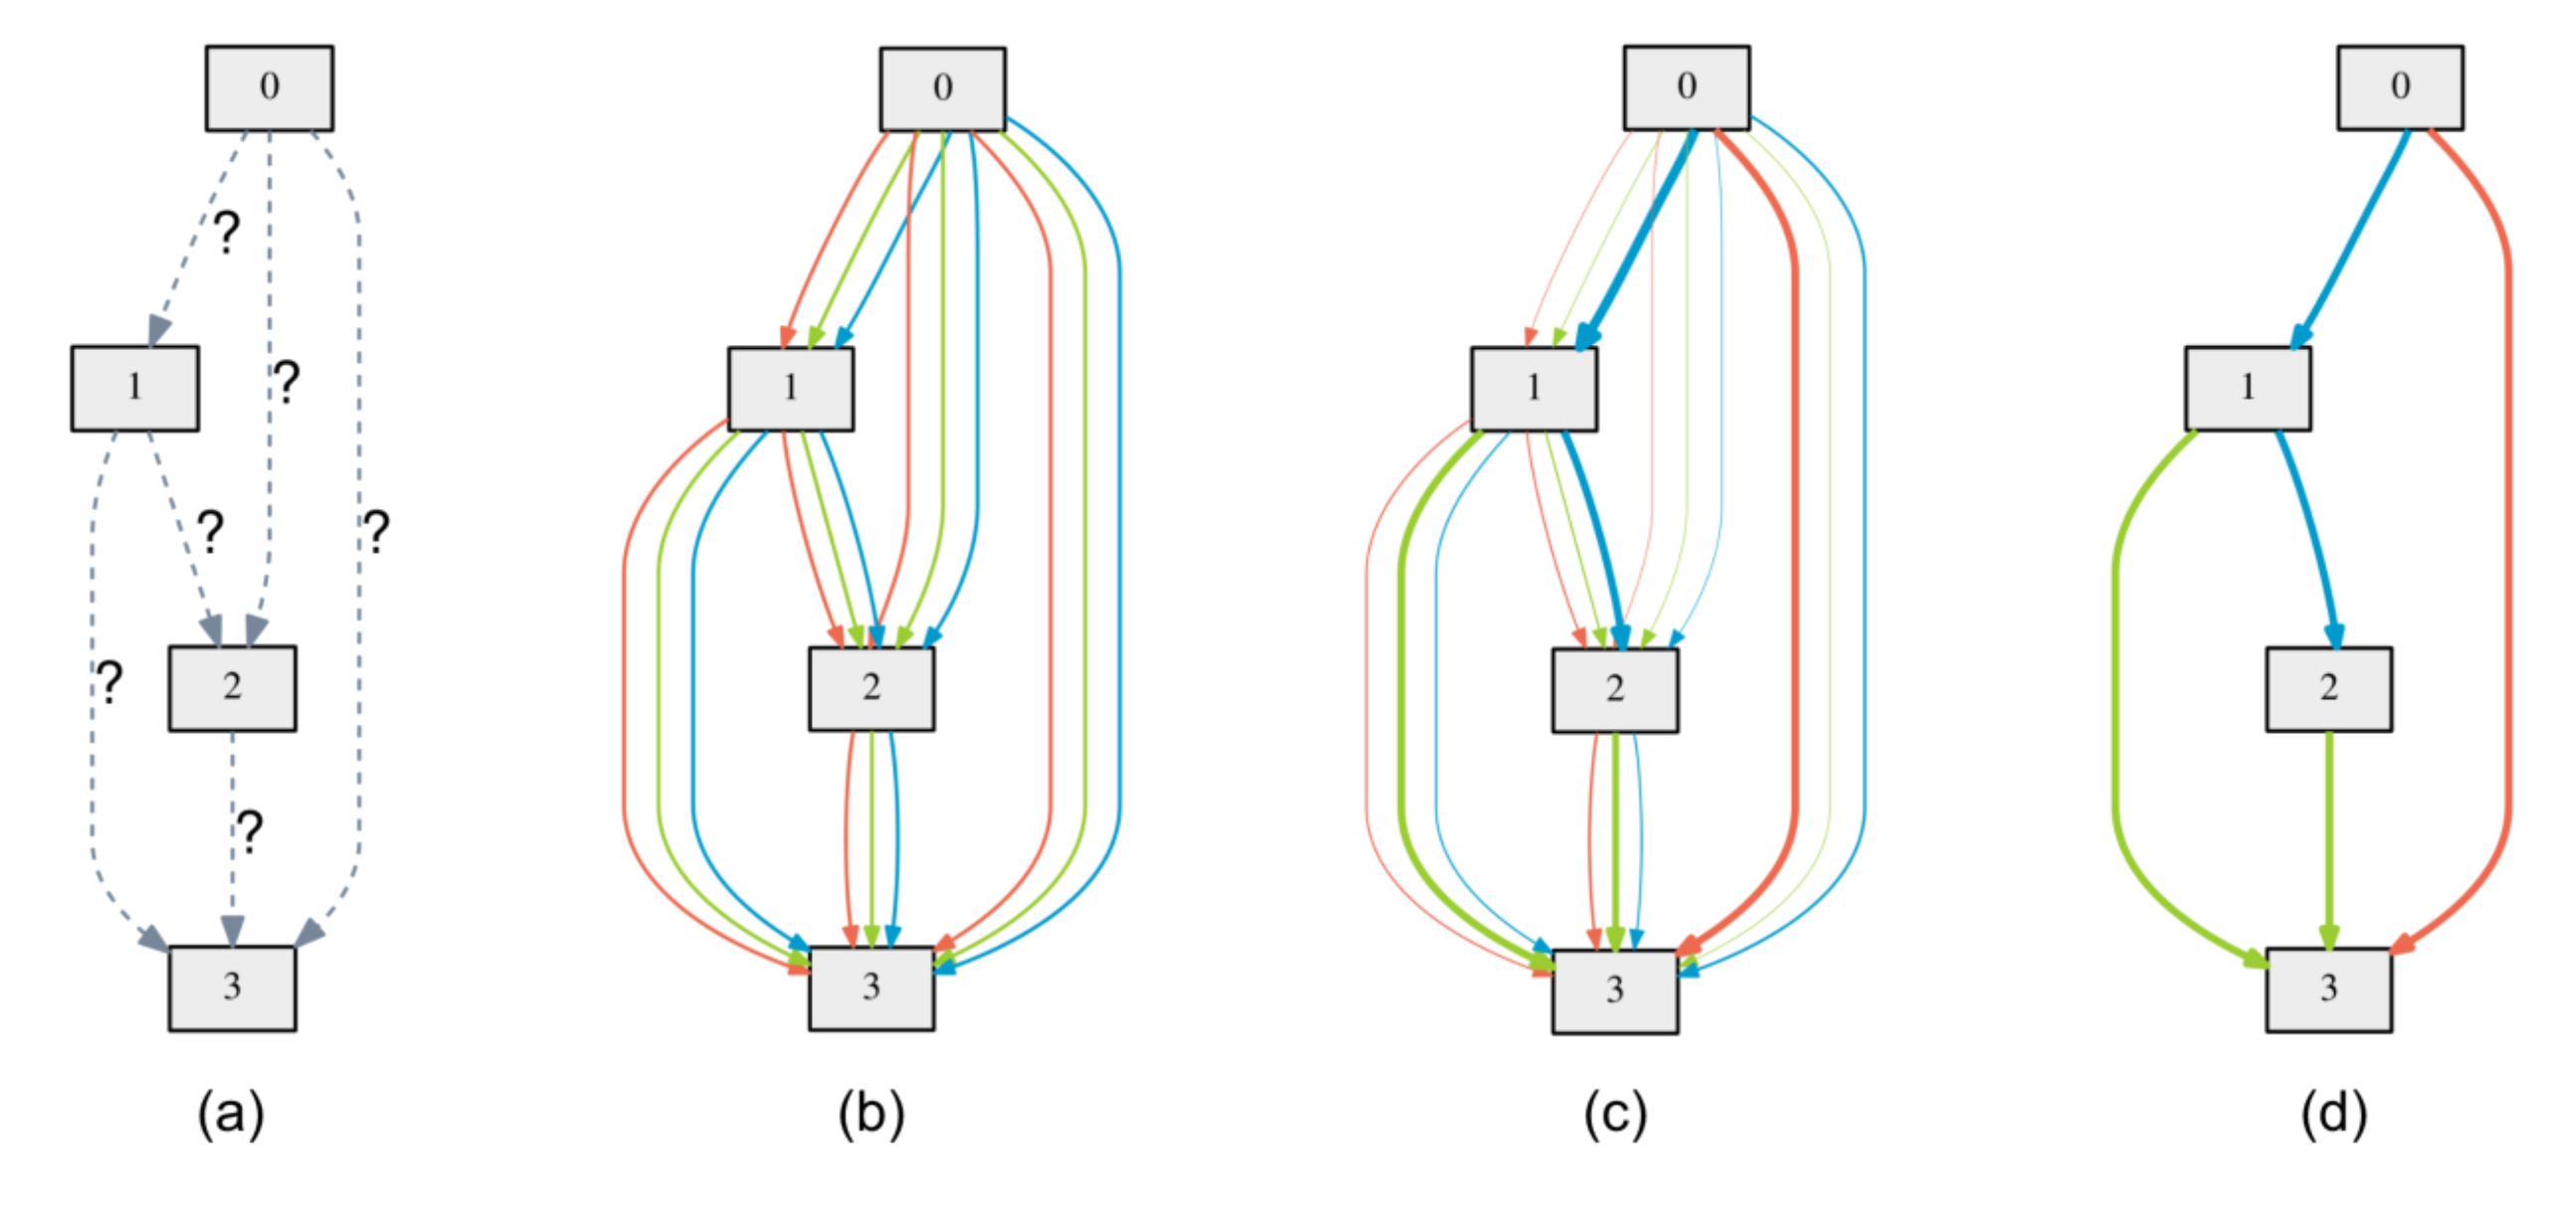
\includegraphics[width=.8\textwidth]{darts.png}\\
                }

            }{
                {\bf Data augmentation:} $\lambda$ parametrizes the transformations distribution. \\

                {\centering
                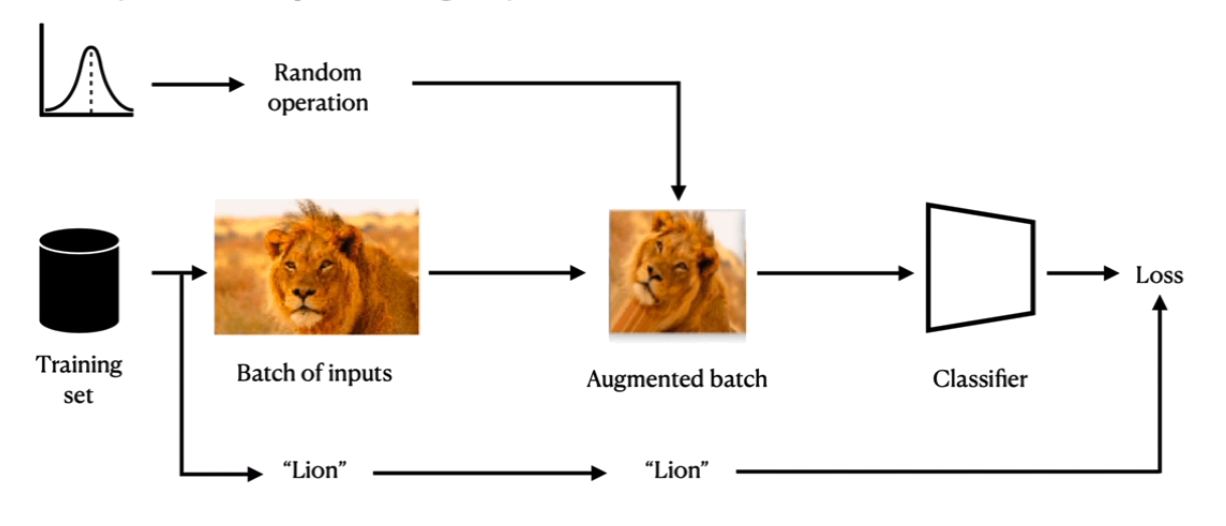
\includegraphics[]{data_aug.png}\\
                }
            }
        }{
            {\bf Hyperparameter optimization:} $\lambda$ is a regularization parameter:\\[1em]

            {\centering
            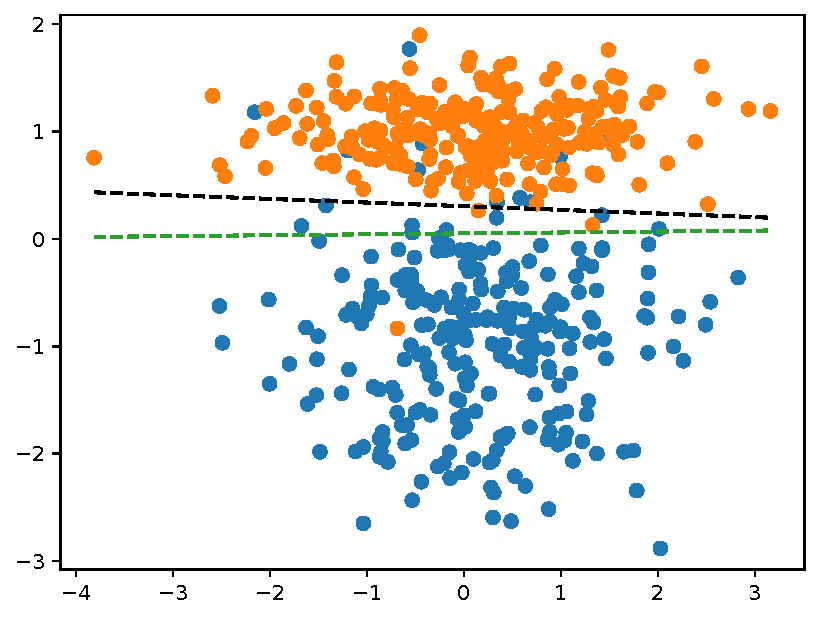
\includegraphics[width=.4\textwidth]{images/logreg_reg}\\
            }
        }

        % \begin{itemize}
        %     \item \emph{Hyperparameter optimization:}
        %         $\lambda$ are the regularisation parameters,\\
        %         or the number of trees, \dots\\
        %         \rightcite{Pedregosa 2016, Lorraine et al. 2020}
        %     \item \emph{Automatic Data Augmentation:} $\lambda$ are the parameters of data augmentation used to train the model.\\
        %     \rightcite{Cubuk et al. 2019; Rommel et al. 2022}
        %     \item \emph{Neural Architecture Search:} $\lambda$ are the parameter of a Neural Network architecture.\\
        %     \rightcite{Liu et al. 2018, Zhang et al. 2021}
        % \end{itemize}

    }


    \frame{
        \frametitle{Bi-level optimization problems: Implicit Deep Learning}

        {\bf Deep Equilibrium Network:}
        \[
            \begin{cases}
            \min_\lambda h(\lambda) = \frac1N\sum_{i=1}^N \mathcal L(y_i, \theta^*(X_i, \lambda))\\
            s.t.\quad \theta^*(X_i, \lambda) = g_\lambda(\theta^*(X_i, \lambda))
            \end{cases}
        \]
        Output of the network is the root of $G(\theta, \lambda) = \theta - g_\lambda(\theta) =0$.\\[2em]

        \begin{columns}
            \column{.4\textwidth}
            \myitem{} {\bf Mimic infinite depth:}
            \[
                \theta^{(t+1)} = g_\lambda(\theta^{(t)})\quad t\to\infty\enspace .
            \]
            \myitem{} {\bf Efficient memory}\\
            \myitem{} {\bf Slow runtime}
            \column{.5\textwidth}
            {\centering
                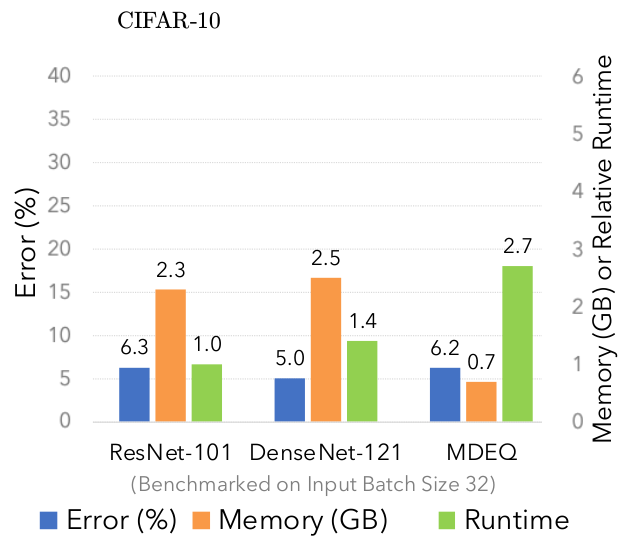
\includegraphics[width=.9\textwidth]{deq_memory.png}\\
            }
        \end{columns}
    }

    \frame{
        \frametitle{Solving bi-level optimization}


        \underline{\bf Black box methods:} Take $\{\lambda_k\}_k$ and compute $\min_k h(\lambda_k)$ \\[1em]
        {
            \centering
            \myitem{} Grid-Search
            \hskip4ex
            \myitem{} Random-Search
            \hskip4ex
            \myitem{} Bayesian-Optimization\\[1em]
        }
        \strongpoint{Do not scale well with the dimension}

        \vskip2em
        \underline{\bf First order methods:} Gradient descent on $h$
        \begin{columns}
            \column{.5\textwidth}
            \vskip1em
            Iterate in the steepest direction:
            $$
                \lambda^{t+1} = \lambda^t - \rho^t \nabla h(\lambda)
            $$
            \myitem{} Gradient $\nabla h(\lambda) = \frac{d\; F(\lambda, \theta^*(\lambda))}{d\;\lambda}$\\[.5em]
            \myitem{} Step size $\rho^t$.
            \column{.5\textwidth}
            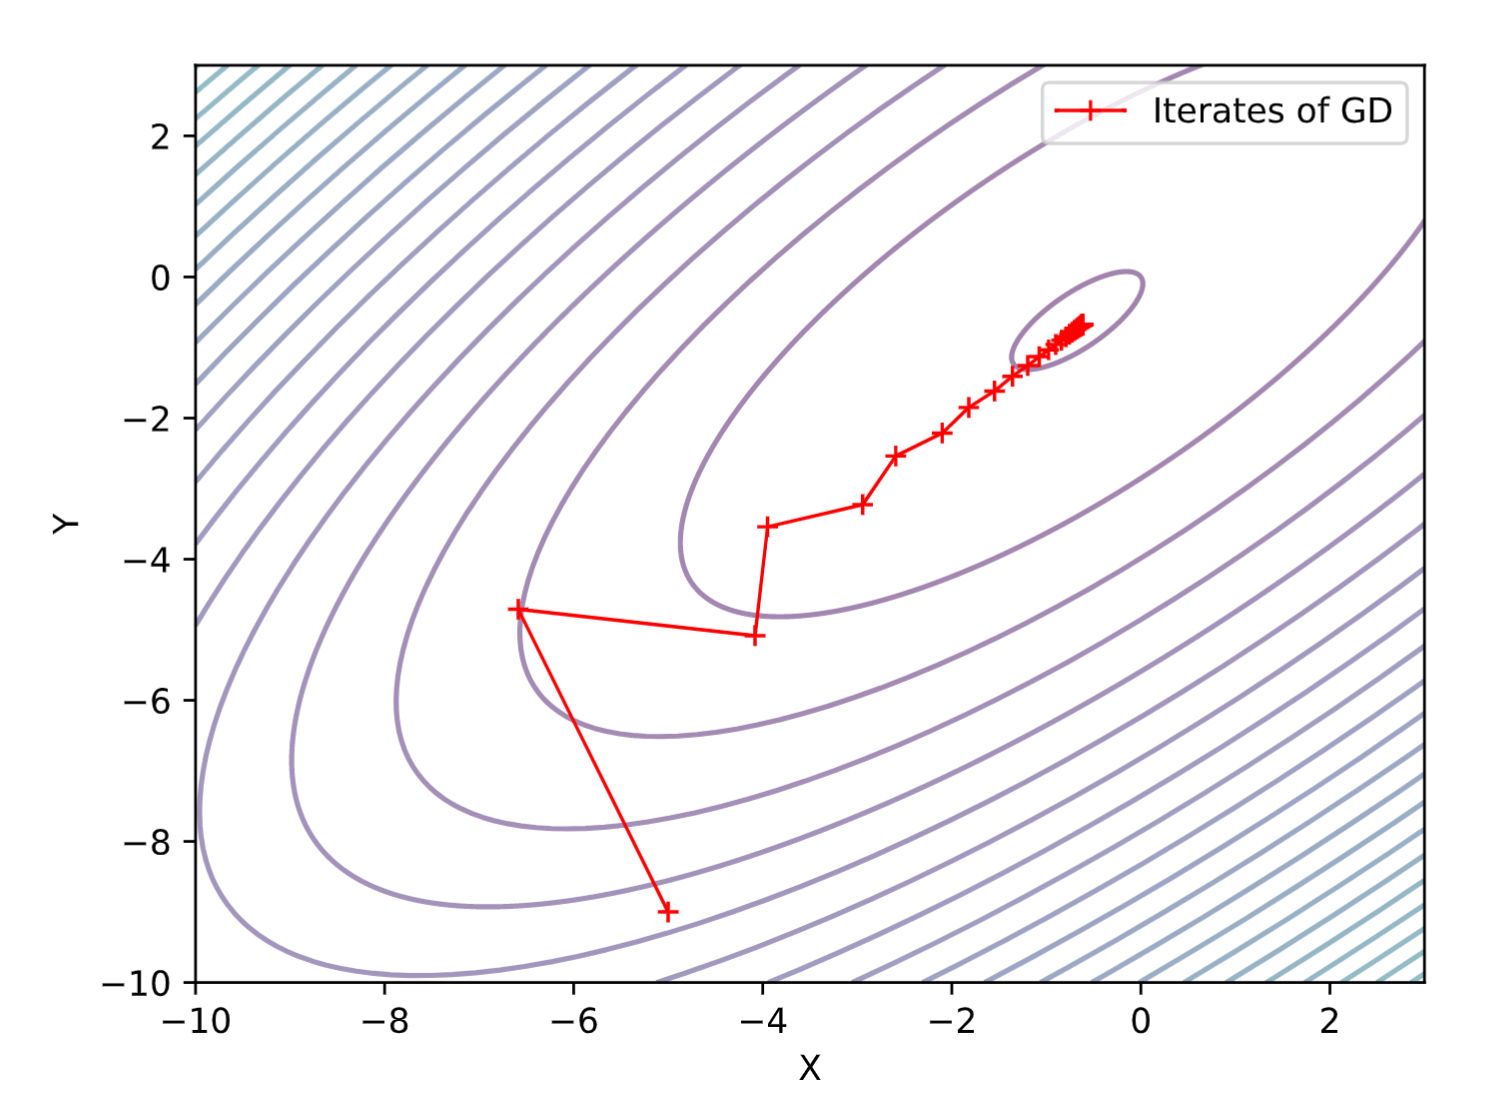
\includegraphics[width=\textwidth]{gd_Steps.png}
        \end{columns}
    }

    \frame{
        \frametitle{Computing the gradient of $h$}

        \underline{\bf{Value function definition:}}
        \[
            h(\lambda) = F(\lambda, \theta^*(\lambda))
        \]

        \underline{\bf{Value function gradient:}}\\[1em]
        \[
            \nabla h(\lambda) = \nabla_1 F(\lambda, {\alt<2>{\color{red}}{}\theta^*})
        -  \nabla_{21}^2 G(\lambda, {\alt<2>{\color{red}}{}\theta^*})
        {\alt<3>{\color{red}}{}
        \big[\nabla_{22}^2G(\lambda, {\alt<2>{\color{red}}{}\theta^*})\big]^{-1}\nabla_2 F(\lambda, {\alt<2>{\color{red}}{}\theta^*})}
        \]

        \vskip1em
        \begin{itemize}\itemsep1em
            \item<2-> Need to compute the solution of the inner
            \item<3-> Need to solve a $p\times p$ linear system
            \only<3>{\[ v^*(\lambda) = \big[\nabla_{22}^2G(\lambda, \theta^*)\big]^{-1}\nabla_2 F(\lambda, \theta^*)\]}
        \end{itemize}
    }

    \section{Approximate bilevel optimization}
    \parttitleframe[Approximating the Hypergradient]{}

    \frame{
        \frametitle{Two-loops approaches}


        {\bf Idea: } Approximate $\theta^*(\lambda^t)$ and $v^*(\lambda^t)$ at each iteration.\\[.5em]


        \visible<2->{
        \begin{itemize}\itemsep.5em
            \item Compute $\theta^t$ such that $\|\theta^t - \theta^*(\lambda^t)\|_2 \le \epsilon_t$, \\
                \keypoint{iterative solver \emph{e.g.} L-BFGS}
            \item Compute hypergradient $g^t = \nabla_1 F(\lambda^t, \theta^t)
            + \nabla^2_{12}G(\lambda^t, \theta^t) v^t$ with $v^t \approx \big[\nabla_{22}^2G(\lambda^t, \theta^t)\big]^{-1}\nabla_2 F(\lambda^t, \theta^t)$ with error $\epsilon_t$,\\
            \keypoint{linear system solver \emph{e.g.} CG}
            % \item Compute the gradient $g_t = $
            \item Update $\lambda^t$ with $\lambda^{t+1} = \lambda^t - \rho^t g^t$.
        \end{itemize}
        }

        \visible<3->{
            \vskip1em
        \begin{theorem}[Two-loops Convergence ; \textcolor{linkcolor}{Pedregosa 2016}]
            If $\sum_t \epsilon_t < \infty$ and the step-sizes are chosen appropriatly, then the algorithm converges to a stationary point of $h$ \emph{i.e.}
       $$
           \|\nabla h(\lambda^t)\|_2 \to 0 \enspace.
       $$
       \end{theorem}
        }
    }

    \frame{
        \frametitle{Further linear system approximation $v^*$}

        Linear system solution $v^*(\lambda^t)$ is a by-product.

        \strongpoint{Avoid computing it as much as possible.}

        \vskip2em
        \underline{\bf Proposed Methods:}\\[1em]
        \begin{columns}[T]
            \column{.4\linewidth}
            \myitem{} Conjugate Gradient\\[1em]
            \myitem{} Jacobian-Free method
            \[
                \phantom{\sum_k}\nabla_{22}^2 G(\lambda^t, \theta^t) \approx Id
            \]\vskip-.5em
            \myitem{} SHINE
            \column{.6\linewidth}
            \myitem{} Algorithm unrolling (\emph{backprop.})\\[1em]
            \myitem{} Neumann iterations
            \[
                \nabla_{22}^2 G(\lambda^t, \theta^t)^{-1}\approx \sum_k (Id - \nabla_{22}^2 G(\lambda^t, \theta^t))^k
            \]
        \end{columns}
        \vspace{0pt plus 1 filll}
        \rightcite{Pedregosa 2016, Lorraine et al. 2020, Luketina et al. 2016, ...}


    }

    % \frame{
    %     \frametitle{Two-loops approaches}

    %     \vskip1em
    %     \underline{Many algorithms developped:}\\[1em]
    %     \myitem{} Warm-start for $\theta^t$ and $v^t$.\\[.5em]
    %     \myitem{} Variance reduction for stochastic algorithms\\[.5em]
    %     \myitem{} Various inverse HVP computation strategies: Neumann/SGD\\[1.5em]

    %     BSA; Stocbio; \dots % XXX:
    % }

    \frame{
        \frametitle{SHINE: SHaring the INverse Estimate
                    \rightcite{Ramzi et al. 2022}}

        \underline{\bf Quasi Newton 101:}\\[1em]
        {\centering Solving $\theta^*(\lambda) = \argmin_\theta G(\lambda, \theta)$\\[2em]}
        \begin{columns}[T]
            \column{.45\linewidth}
            {\centering \bf Newton Method\\}
            \[
                \theta^{t+1} = \theta^t - \big[\nabla^2G(\theta^t)\big]^{-1}\nabla G(\theta^t)
            \]

            \column{.55\linewidth}
            {\centering \bf Quasi-Newton Method\\[.7em]}
            \[
                \theta^{t+1} = \theta^t - B_t^{-1}\nabla G(\theta^t)
            \]
            $B_t^{-1}$: low-rank approx. of $\nabla^2G(\theta^t)^{-1}$.
        \end{columns}

        \pause
        \vskip1em
        \strongpoint{
            \textbf{SHINE} propose to use $B_t^{-1}$ to approximate $v^*(\lambda^t)$
            $$
                g^t = \nabla_1 F(\lambda^t, \theta^t)
            + \nabla^2_{12}G(\lambda^t, \theta^t) B_t^{-1} \nabla_2 F(\lambda^t, \theta^t)
            $$
        }
    }

    \frame{
        \frametitle{SHINE - Hyperparameter optimization \rightcite{Ramzi et al. 2022}}

        Logistic Regression with $\ell_2$-regularisation on 2 datasets:\\[1em]

        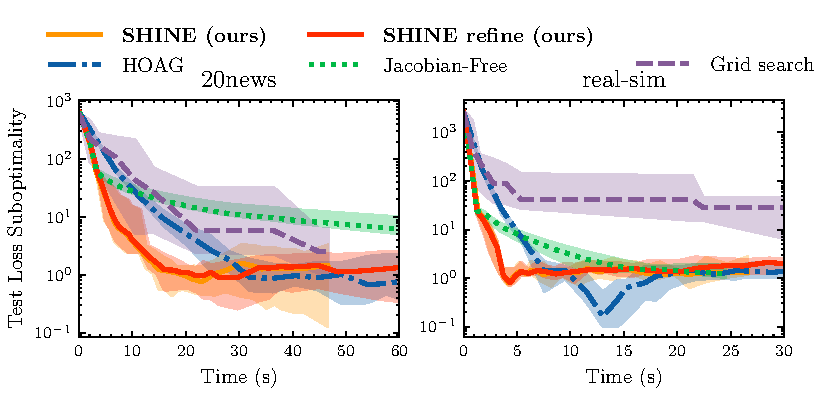
\includegraphics[width=\textwidth]{bilevel_test.pdf}\\
    }
    % \frame{
    %     \frametitle{SHINE - DEQ \rightcite{Ramzi et al. 2022}}

    %     Multiscale DEQ on CIFAR10:\\[1em]

    %     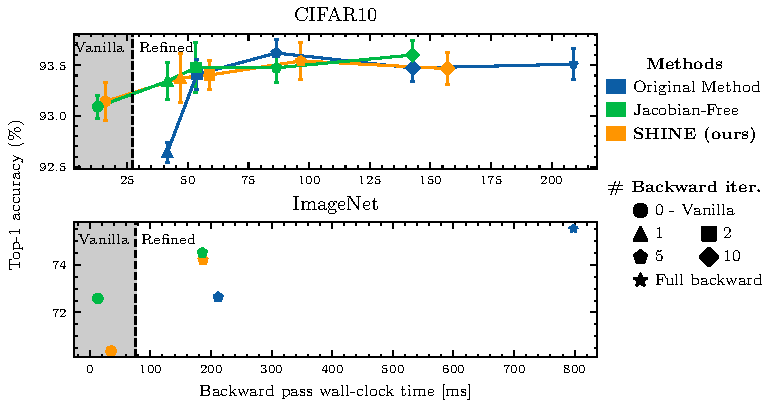
\includegraphics[width=\textwidth]{mdeq.pdf}\\
    % }

    \section{Stochastic Bilevel Optimization}
    \parttitleframe[]{}

    \frame{
        \frametitle{Stochastic bilevel optimization}

        $$F(\lambda, \theta) = \frac1m\sum_{j=1}^m F_j(\lambda, \theta),\quad G(\lambda, \theta) = \frac1n\sum_{i=1}^n G_i(\lambda, \theta)$$

        \visible<2->{
            \textbf{Stochastic updates:}\\[1em]

            \begin{itemize}
                \item Compute $\theta^t$ with SGD,\\[.5em]
                \item Compute stochastic $g^t = \nabla_1 F_j(\lambda^t, \theta^t)
                + \nabla^2_{12}G_i(\lambda^t, \theta^t) v^t$ with $v^t \approx \big[\nabla_{22}^2G_i(\lambda^t, \theta^t)\big]^{-1}\nabla_2 F_j(\lambda^t, \theta^t)$,\\[.5em]
                \item Update $\lambda^t$ with $g^t$.\\[.5em]
            \end{itemize}

        }

        \visible<3->{
        \vspace{.4cm}
        \textbf{Problem:}
        $$
        \left[\sum_{i=1}^n\nabla^2_{22} G_i(\lambda, \theta^*(\lambda))\right]^{-1}\neq\sum_{i=1}^n\left[\nabla^2_{22} G_i(\lambda, \theta^*(\lambda))\right]^{-1}
        $$
        }

}


\begin{frame}{Stochastic linear system resolution}
    Stochastic approximation of $v^t = \left[\nabla^2_{22} G(\lambda^t, \theta^t)\right]^{-1}\nabla_2 F_j(\lambda^t, \theta^t)$.

    \vspace{.5cm}
    \begin{itemize}[<+->]
        \item Neumann approximations \citeline{Ghadimi et al. 2018, Ji et al. 2021}:

        $$
        v^t
        \approx
        \eta\sum_{q=0}^{Q
        }
        \prod_{k=0}^q\left(I - \eta\nabla^2_{22}G_{i_k}(\lambda^t, \theta^t)\right)\nabla_2 F_j (\lambda^t, \theta^t)
        $$

        % \only<2->{
        % $$v^t \approx \sum_{q=0}^Q\prod_{k=0}^q\left(I - \nabla^2_{11}G_{i_k}(\theta^t, \lambda^t)\right)\nabla_1 F_j(\theta^t, \lambda^t)$$
        % }

        \vspace{.3cm}
        \item Stochastic Gradient Descent \citeline{Grazzi et al. 2021, Arbel et al. 2021}
        $$v^t \in \argmin_{v\in\mathbb R^p} \frac1n\sum_{i=1}^n\frac12\langle \nabla^2_{22} G_i(\lambda^t, \theta^t)v, v\rangle + \frac1n\sum_{j=1}^m\langle \nabla_2 F_j(\lambda^t, \theta^t), v\rangle$$
    \end{itemize}

    \pause
    \strongpoint{Still need to solve 2 optimization problems for\\every updates on the outer variable.}
\end{frame}


\section{One-loop Approaches}
\parttitleframe[Toward linear updates]{Dagreou2022,Dagreou2023}

% \frame{

%     \frametitle{First approaches to one-loop algorithms}
%     Alternate steps in $\theta$ and $\lambda$ \citeline{Hong et al. 2020, Yang et al. 2021}:

%     \vspace{.3cm}
%     \begin{align*}
%         \theta^{t+1} &= \theta^t - \rho^t\nabla_2 G_i (\lambda^t, \theta^t)\quad\text{\textcolor{black!50}{SGD step}}\\
%         v^{t+1} &= \eta\sum_{q=1}^Q\prod_{k=0}^q\left(I-\eta\nabla^2_{22} G_{i_k}(\lambda^t, \theta^{t+1})\right) \nabla_2 F_j(\lambda^t, \theta^{t+1})\\&\hskip15em\text{\textcolor{black!50}{Neumann approximation}}\\
%         \lambda^{t+1} &= \lambda^t - \gamma^t(\underbrace{\nabla_1 F_j(\lambda^t, \theta^{t+1})-\nabla^2_{12}G_i(\lambda^t, \theta^{t+1})v^{t+1}}_{\approx \nabla h(\lambda^t)})
%     \end{align*}


% }

\begin{frame}{Main idea}
    Three variables to maintain:
    \begin{itemize}
        \item $\theta^t\rightarrow$ solution to the inner problem
        \item $v^t\rightarrow$ solution of the linear system
        \item $\lambda^t\rightarrow$ solution of the outer problem
    \end{itemize}

    \vspace{.5cm}
    \textbf{Idea:} evolve in $\theta^t$, $v^t$ and $\lambda^t$ at the same time following well chosen directions.
\end{frame}


\begin{frame}{Motivation of the framework}

\textbf{Update directions: }
\begin{align*}
    \visible<1->{D_\theta(\theta, v, \lambda) &= \nabla_2 G(\lambda, \theta)\quad\text{\textcolor{black!50}{gradient step toward $\theta^*(\lambda)$}}} \\
    \visible<2->{D_v(\theta, v, \lambda) &= \nabla^2_{22} G(\lambda, \theta)v + \nabla_2 F(\lambda, \theta)\\&\text{\textcolor{black!50}{gradient step toward $-\left[\nabla^2_{11} G(\lambda, \theta)\right]^{-1}\nabla_2 F(\lambda, \theta)$}}} \\
    \visible<3->{D_\lambda(\theta, v, \lambda) &= \nabla^2_{12} G(\lambda, \theta)v + \nabla_1 F(\lambda, \theta)\\&\text{\textcolor{black!50}{gradient step toward $\lambda^*$}}}
\end{align*}



\visible<4->{
    \vskip1em
    \textbf{\underline{Algorithm}}\\
    \centering
    \parbox{.8\textwidth}{
        For $t=1...T$:
        \begin{enumerate}
            \item Update $\theta^{t+1} = \theta^t - \rho^t D^t_\theta$
            \item Update $v^{t+1} = v^t - \rho^t D^t_v$
            \item Update $\lambda^{t+1} = \lambda^t - \gamma^t D^t_\lambda$
        \end{enumerate}
    }\\
}
\end{frame}

\begin{frame}{Motivation of the framework}
\textbf{Stochastic Update Directions: }
    \begin{align*}
        D_\theta(\theta, v, \lambda) &= \frac1n\sum_{i=1}^n\nabla_2 G_i(\lambda, \theta) \\
        D_v(\theta, v, \lambda) &= \frac1n\sum_{i=1}^n\nabla^2_{22} G_i(\lambda, \theta)v + \frac1m\sum_{j=1}^m\nabla_2 F_j(\lambda, \theta) \\
        D_\lambda(\theta, v, \lambda) &= \frac1n\sum_{i=1}^n\nabla^2_{12} G_i(\lambda, \theta)v + \frac1m\sum_{j=1}^m\nabla_1 F_j(\lambda, \theta)
    \end{align*}

    \strongpoint{Additive expressions with natural stochastic estimators.}

\end{frame}



\begin{frame}{SOBA (StOchastic Bilevel Algorithm) directions}
    Pick $i\in\{1,\dots,n\}$ and $j\in\{1,\dots,m\}$ and take
    \vspace{.5cm}
    \begin{align*}
        D_\theta^t &= \nabla_2 G_i(\lambda^t, \theta^t) \\
        D_v^t &= \nabla^2_{22} G_i(\lambda^t, \theta^t)v^t + \nabla_2 F_j(\lambda^t, \theta^t) \\
        D_\lambda^t &= \nabla^2_{12} G_i(\lambda^t, \theta^t)v^t + \nabla_1 F_j(\lambda^t, \theta^t)
    \end{align*}
\end{frame}

% \begin{frame}{SOBA (StOchastic Bilevel Algorithm) directions}
%     \begin{align*}
%         \mathbb E_{i,j}[D_\theta^t] &= \frac1n\sum_{i=1}^n\nabla_2 G_i(\lambda^t, \theta^t) = D_\theta(\theta^t, v^t, \lambda^t) \\
%         \mathbb E_{i,j}[D_v^t] &= \frac1n\sum_{i=1}^n\nabla^2_{22} G_i(\lambda^t, \theta^t)v^t + \frac1m\sum_{j=1}^m\nabla_2 F_j(\lambda^t, \theta^t) = D_v(\theta^t, v^t, \lambda^t) \\
%         \mathbb E_{i,j}[D_\lambda^t] &= \frac1n\sum_{i=1}^n\nabla^2_{12} G_i(\lambda^t, \theta^t)v^t + \frac1m\sum_{j=1}^m\nabla_1 F_j(\lambda^t, \theta^t) = D_\lambda(\theta^t, v^t, \lambda^t)
%     \end{align*}
% \end{frame}

\begin{frame}{Theoretical guarantees of SOBA}
    \begin{theorem}[Convergence of SOBA]
        Under some regularity assumptions on $F$ and $G$, if $h$ is bounded, then for decreasing step sizes that verify $\rho^t = \alpha t^{-\frac25}$ and $\gamma^t = \beta t^{-\frac35}$ for some $\alpha, \beta>0$, the iterates $(\lambda^t)_{1\leq t\leq T}$ of SOBA verify
        $$
        \inf_{t\leq T} \mathbb E[\|\nabla h(\lambda^t)\|^2] = \mathcal O(T^{-\frac12})\enspace .
        $$
    \end{theorem}
\end{frame}


\begin{frame}{Variance-reduced solvers \rightcite{Dagréou et al. 2022, 2023}}

    Natural adaptation of single level stochastic algorithms:\\[1em]
    \begin{itemize}[<+->]
        \item[] \textbf{SABA:} Adaption of SAGA \citeline{Defazio et al. 2014}:\\[.5em]
        The varianced reduced stochastic gradient estimate is:
            $$
            \nabla_2G(\lambda^t, \theta^t) = \nabla_2 G_i(\lambda^t, \theta^t) - \nabla_2 G_i(\lambda^{t_i}, \theta^{t_i}) + \frac1n\sum_{k=1}^n \nabla_2 G_k(\lambda^{t_k}, \theta^{t_k}))
            $$
        \item[] \textbf{SRBA:} Adaption of SARHA \citeline{Nguyen et al. 2017}\\[.5em]
        The varianced reduced stochastic gradient estimate is:
            $$
            \nabla_2G(\lambda^t, \theta^t) = \nabla_2 G_i(\lambda^t, \theta^t) - \nabla_2 G_i(\lambda^{t-1}, \theta^{t-1}) + \nabla_2 G(\lambda^{T_t}, \theta^{T_t})
            $$
    \end{itemize}

    \visible<3->{
        \vskip.5em
        Similar updates for the 5 quantities:
        \begin{gather*}
            \nabla_2 G(\lambda^t, \theta^t),\quad \nabla_2 F(\lambda^t, \theta^t),\quad \nabla_1 F(\lambda^t, \theta^t)\\
            \nabla_{12}^2G(\lambda^t, \theta^t)v^t,\quad\nabla_{22}^2G(\lambda^t, \theta^t) v^t
        \end{gather*}
    }

\end{frame}

% \begin{frame}{Aside: SAGA for single level problems \citeline{Defazio et al. 2014}}
%     \textbf{Single level problem:}
%     $$\min_{\theta\in\mathbb R^p} f(\theta) = \frac1n\sum_{i=1}^n f_i(\theta)$$

%     \pause
%     \textbf{Initialisation: } Compute and store $m[i] = \nabla f_i(\theta^0)$ for any $i\in\{1,\dots,n\}$ and $S[m] = \frac1n\sum_{i=1}^n m[i]$.

%     \pause
%     \textbf{At iteration $t$:}
%     \begin{enumerate}
%         \item Pick $i\in\{1,\dots,n\}$
%         \item Update $\theta$
%         $$\theta^{t+1} = \theta^t - \rho (\nabla f_i(\theta^t) \underbrace{- m[i] + S[m]}_{\text{variance reduction}}) $$
%         \item Update the memory
%         $$m[i] \leftarrow \nabla f_i(\theta^t)$$
%     \end{enumerate}
% \end{frame}


\begin{frame}{Theoretical guarantees \rightcite{Dagréou et al. 2022, 2023}}

    We denote $N = m + n$

    \begin{theorem}[Sample complexity of SABA]
        Under some regularity assumptions on $F$ and $G$, with constant and small enough step sizes, SABA achieves an $\epsilon$-stationary point with a sample complexity of $\mathcal O(N^{\frac23}\epsilon^{-1})$.
    \end{theorem}

    \begin{theorem}[Sample complexity of SRBA]
        Under some regularity assumptions on $F$ and $G$, with constant and small enough step sizes, SRBA achieves an $\epsilon$-stationary point with a sample complexity of $\mathcal O(N^{\frac12}\epsilon^{-1})$.
    \end{theorem}

    \strongpoint{This matches the sample complexity of single level algorithms.}
    \strongpoint{We show that SRBA is near-optimal for a class of bilevel problems.}

\end{frame}

% \begin{frame}{Remarks}
%     \begin{columns}
%         \column{.5\textwidth}
%             \begin{itemize}
%                 \item We match the convergence rate of gradient descent

%                 \vspace{ .5cm}
%                 \item SABA converges with fixed step sizes

%                 \vspace{.5cm}
%                 \item Faster than SOBA
%             \end{itemize}
%         \column{.5\textwidth}
%         \begin{figure}
%         \centering
%         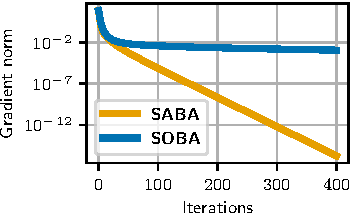
\includegraphics{images/toy.pdf}
%     \end{figure}
%     \end{columns}

% \end{frame}

% \begin{frame}{Complexity}
%     Number of calls to oracle to get an $\epsilon$-stationary solution.

%     \vspace{.5cm}
%     \begin{table}
%         \begin{tabular}{|c|c|c|c|c|>{\columncolor{green!10}}c|>{\columncolor{green!10}}c|}
%             \hline
%             amIGO & stoBiO & TTSA & MRBO & SUSTAIN & \bf SOBA & \bf SABA\\
%             \hline
%             $\mathcal O(\epsilon^{-2})$ & $\tilde{\mathcal O}(\epsilon^{-2})$ & $\tilde{\mathcal O}(\epsilon^{-5/2})$ & $\tilde{\mathcal O}(\epsilon^{-3/2})$ & \bf $\mathcal O(\epsilon^{-3/2})$ & $\mathcal O(\epsilon^{-5/2})$ & $\mathcal O(\epsilon^{-1})$ \\
%             \hline
%         \end{tabular}

%     \vspace{1cm}
%     \centering
%     \bf
%     \red{SABA achieves SOTA complexity}
%     \end{table}


% \end{frame}



\begin{frame}{Hyperparameter selection on $\ell^2$ regularized logistic regression}

    \textbf{Setting: }
    \begin{itemize}
        \item Task: binary classification

        \item IJCNN1 dataset: $49\,990$ training samples, $91\,701$ validation samples, 22 features

        \item Training loss:
           $$G(\theta, \lambda) = \frac1n\sum_{i=1}^n \log(1+\exp(-y_i\langle x_i, \theta\rangle) + \frac12\sum_{k=1}^p e^{\lambda_k}\theta_k^2$$

        \item Validation loss: logistic loss
        $$
        F(\theta, \lambda) = \frac1m\sum_{j=1}^m \log(1+\exp(-y_i^{val}\langle x_i^{val}, \theta\rangle)
        $$
    \end{itemize}

\end{frame}

\begin{frame}{Hyperparameter selection on $\ell^2$ regularized logistic regression}

    \centering
    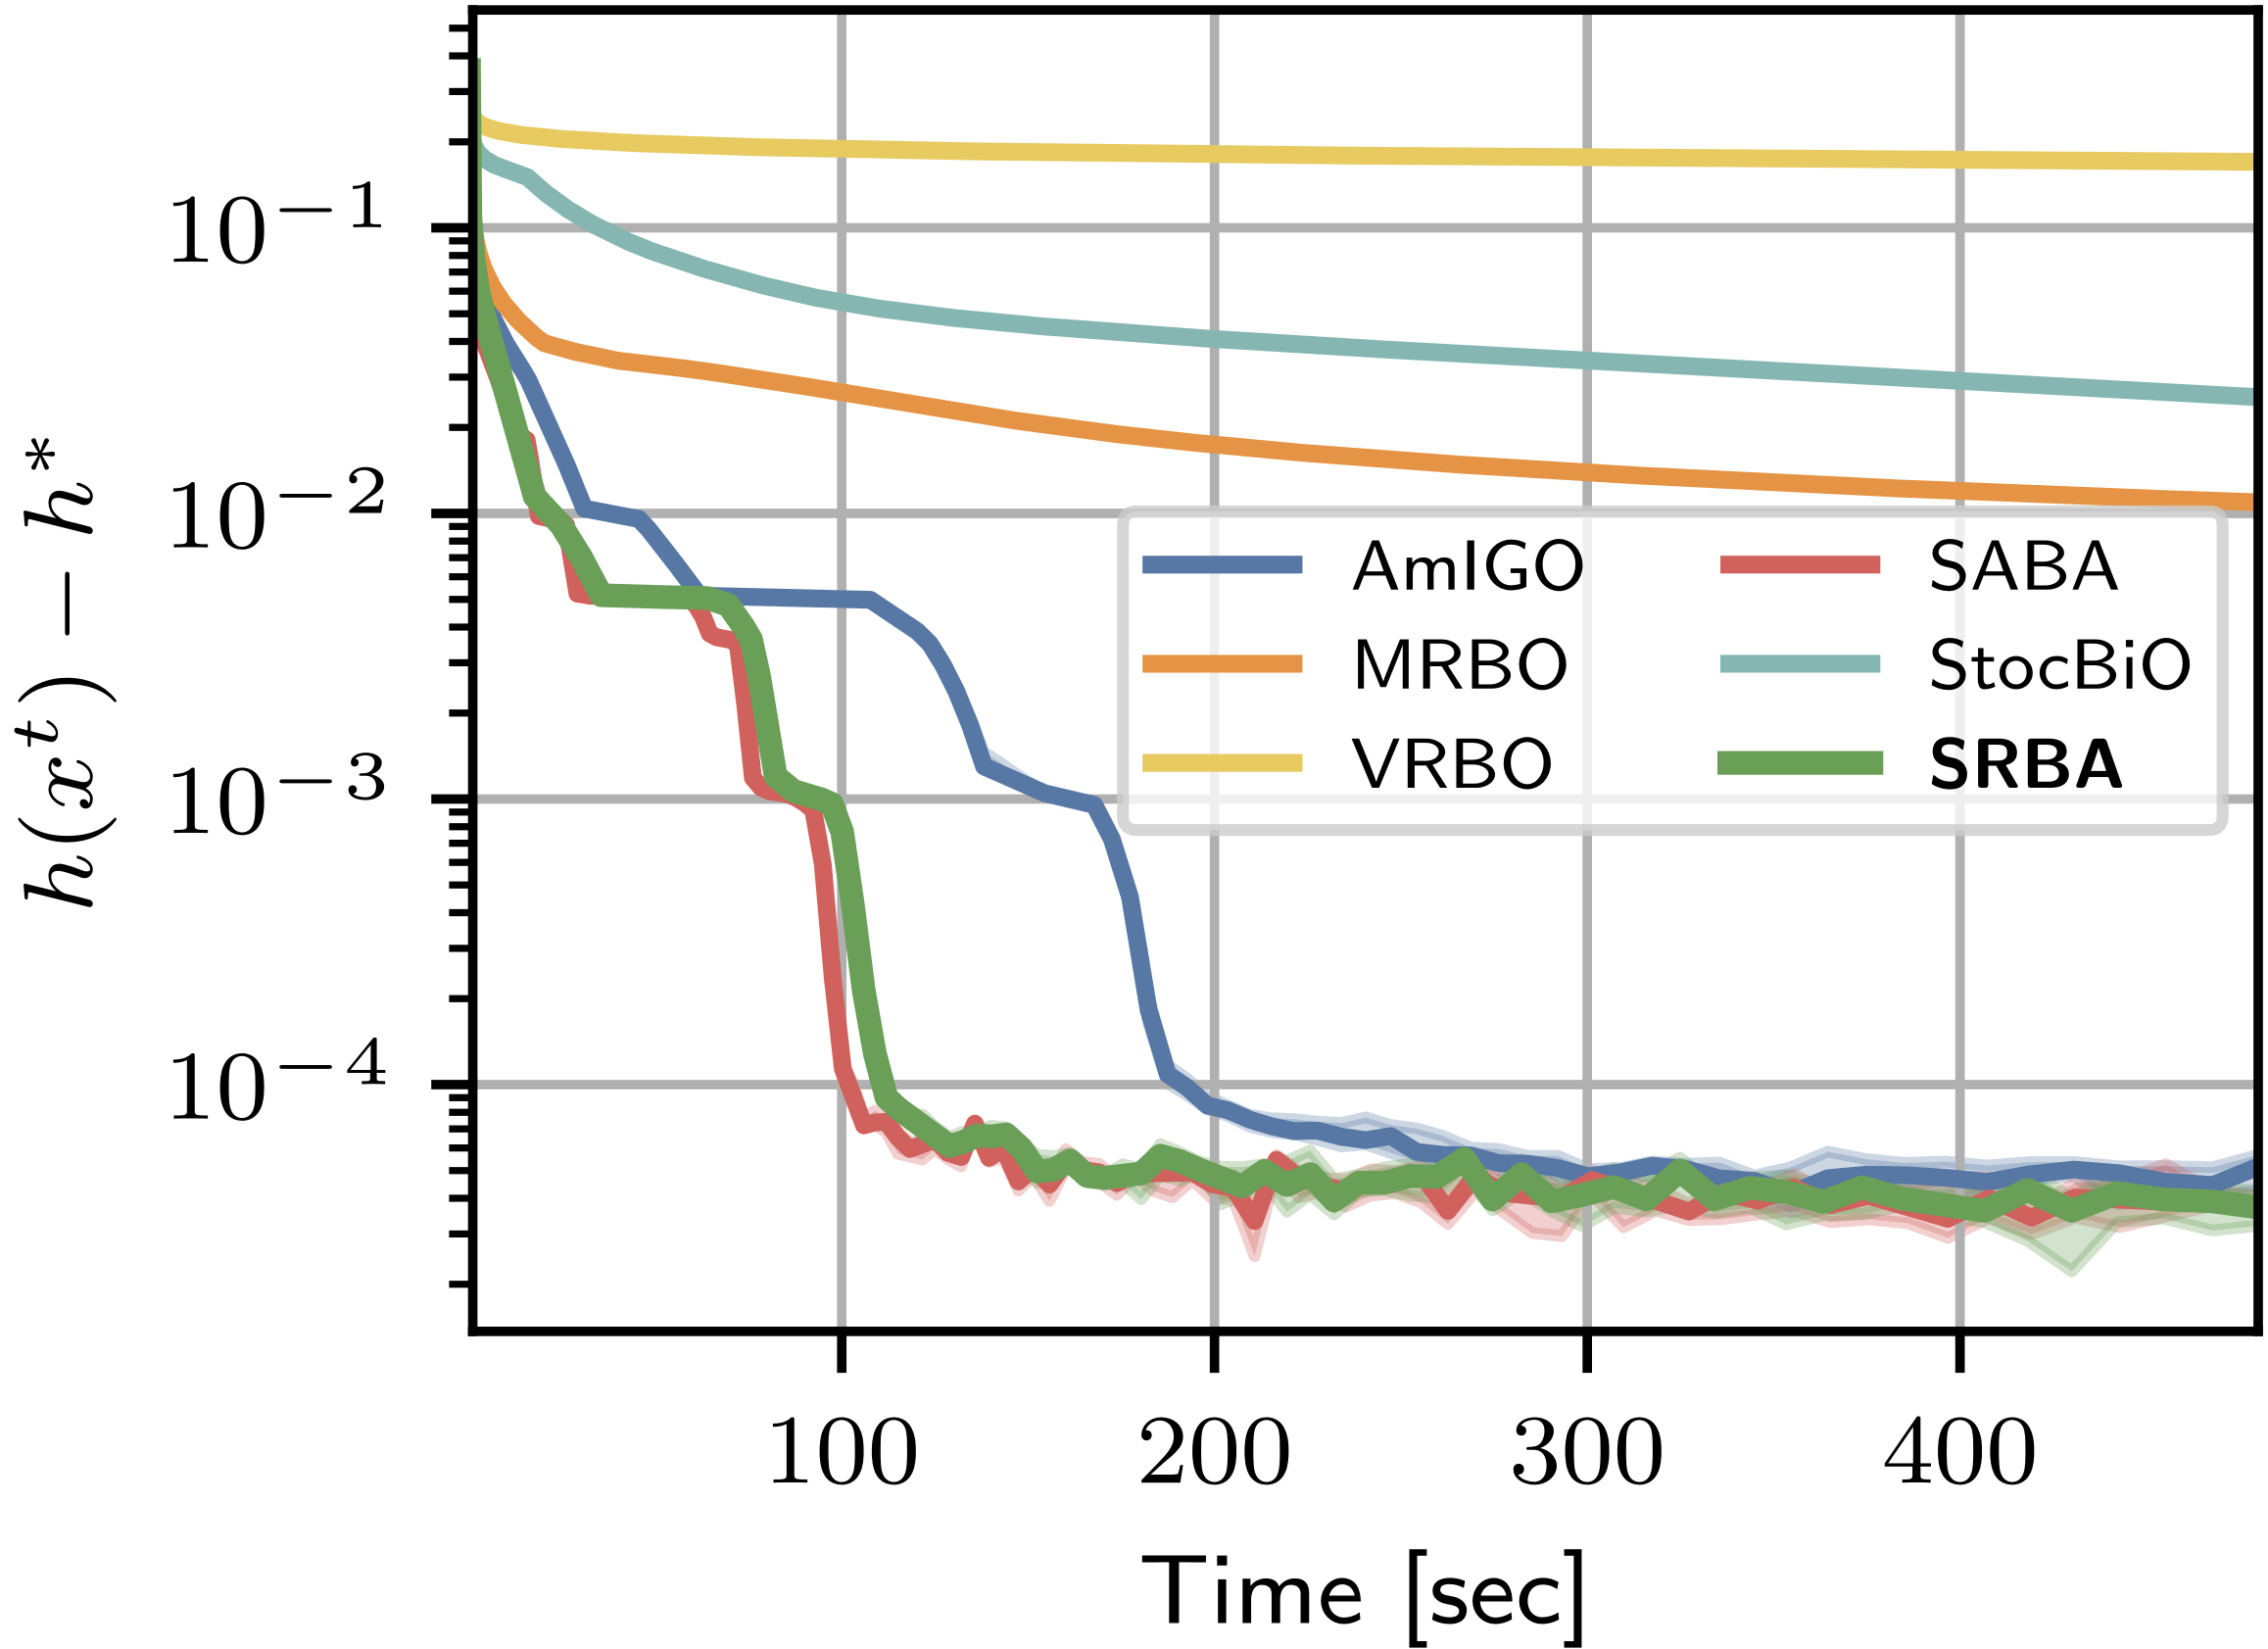
\includegraphics[width=.8\textwidth]{images/SRBA}\\

\end{frame}


%%%%%%%%%%%%%%%%%%%%%%%%%%%%%%%%%%%%%%%%%%%%%%%%%%%%%%%%%%%%%%%%%%%%%%%%%%%%%%%
\begin{frame}[fragile]{Benchopt \rightcite{Moreau et al. 2022}}

Reproducing this comparison and adding solvers and tasks is easy as:\\[.5em]


\begin{center}
\begin{tabular}{c}
\begin{lstlisting}[language=bash,linewidth=.85\textwidth]
git clone https://github.com/benchopt/benchmark_bilevel
benchopt run ./benchmark_bilevel
\end{lstlisting}
\end{tabular}
\end{center}

\vskip.5em\centering
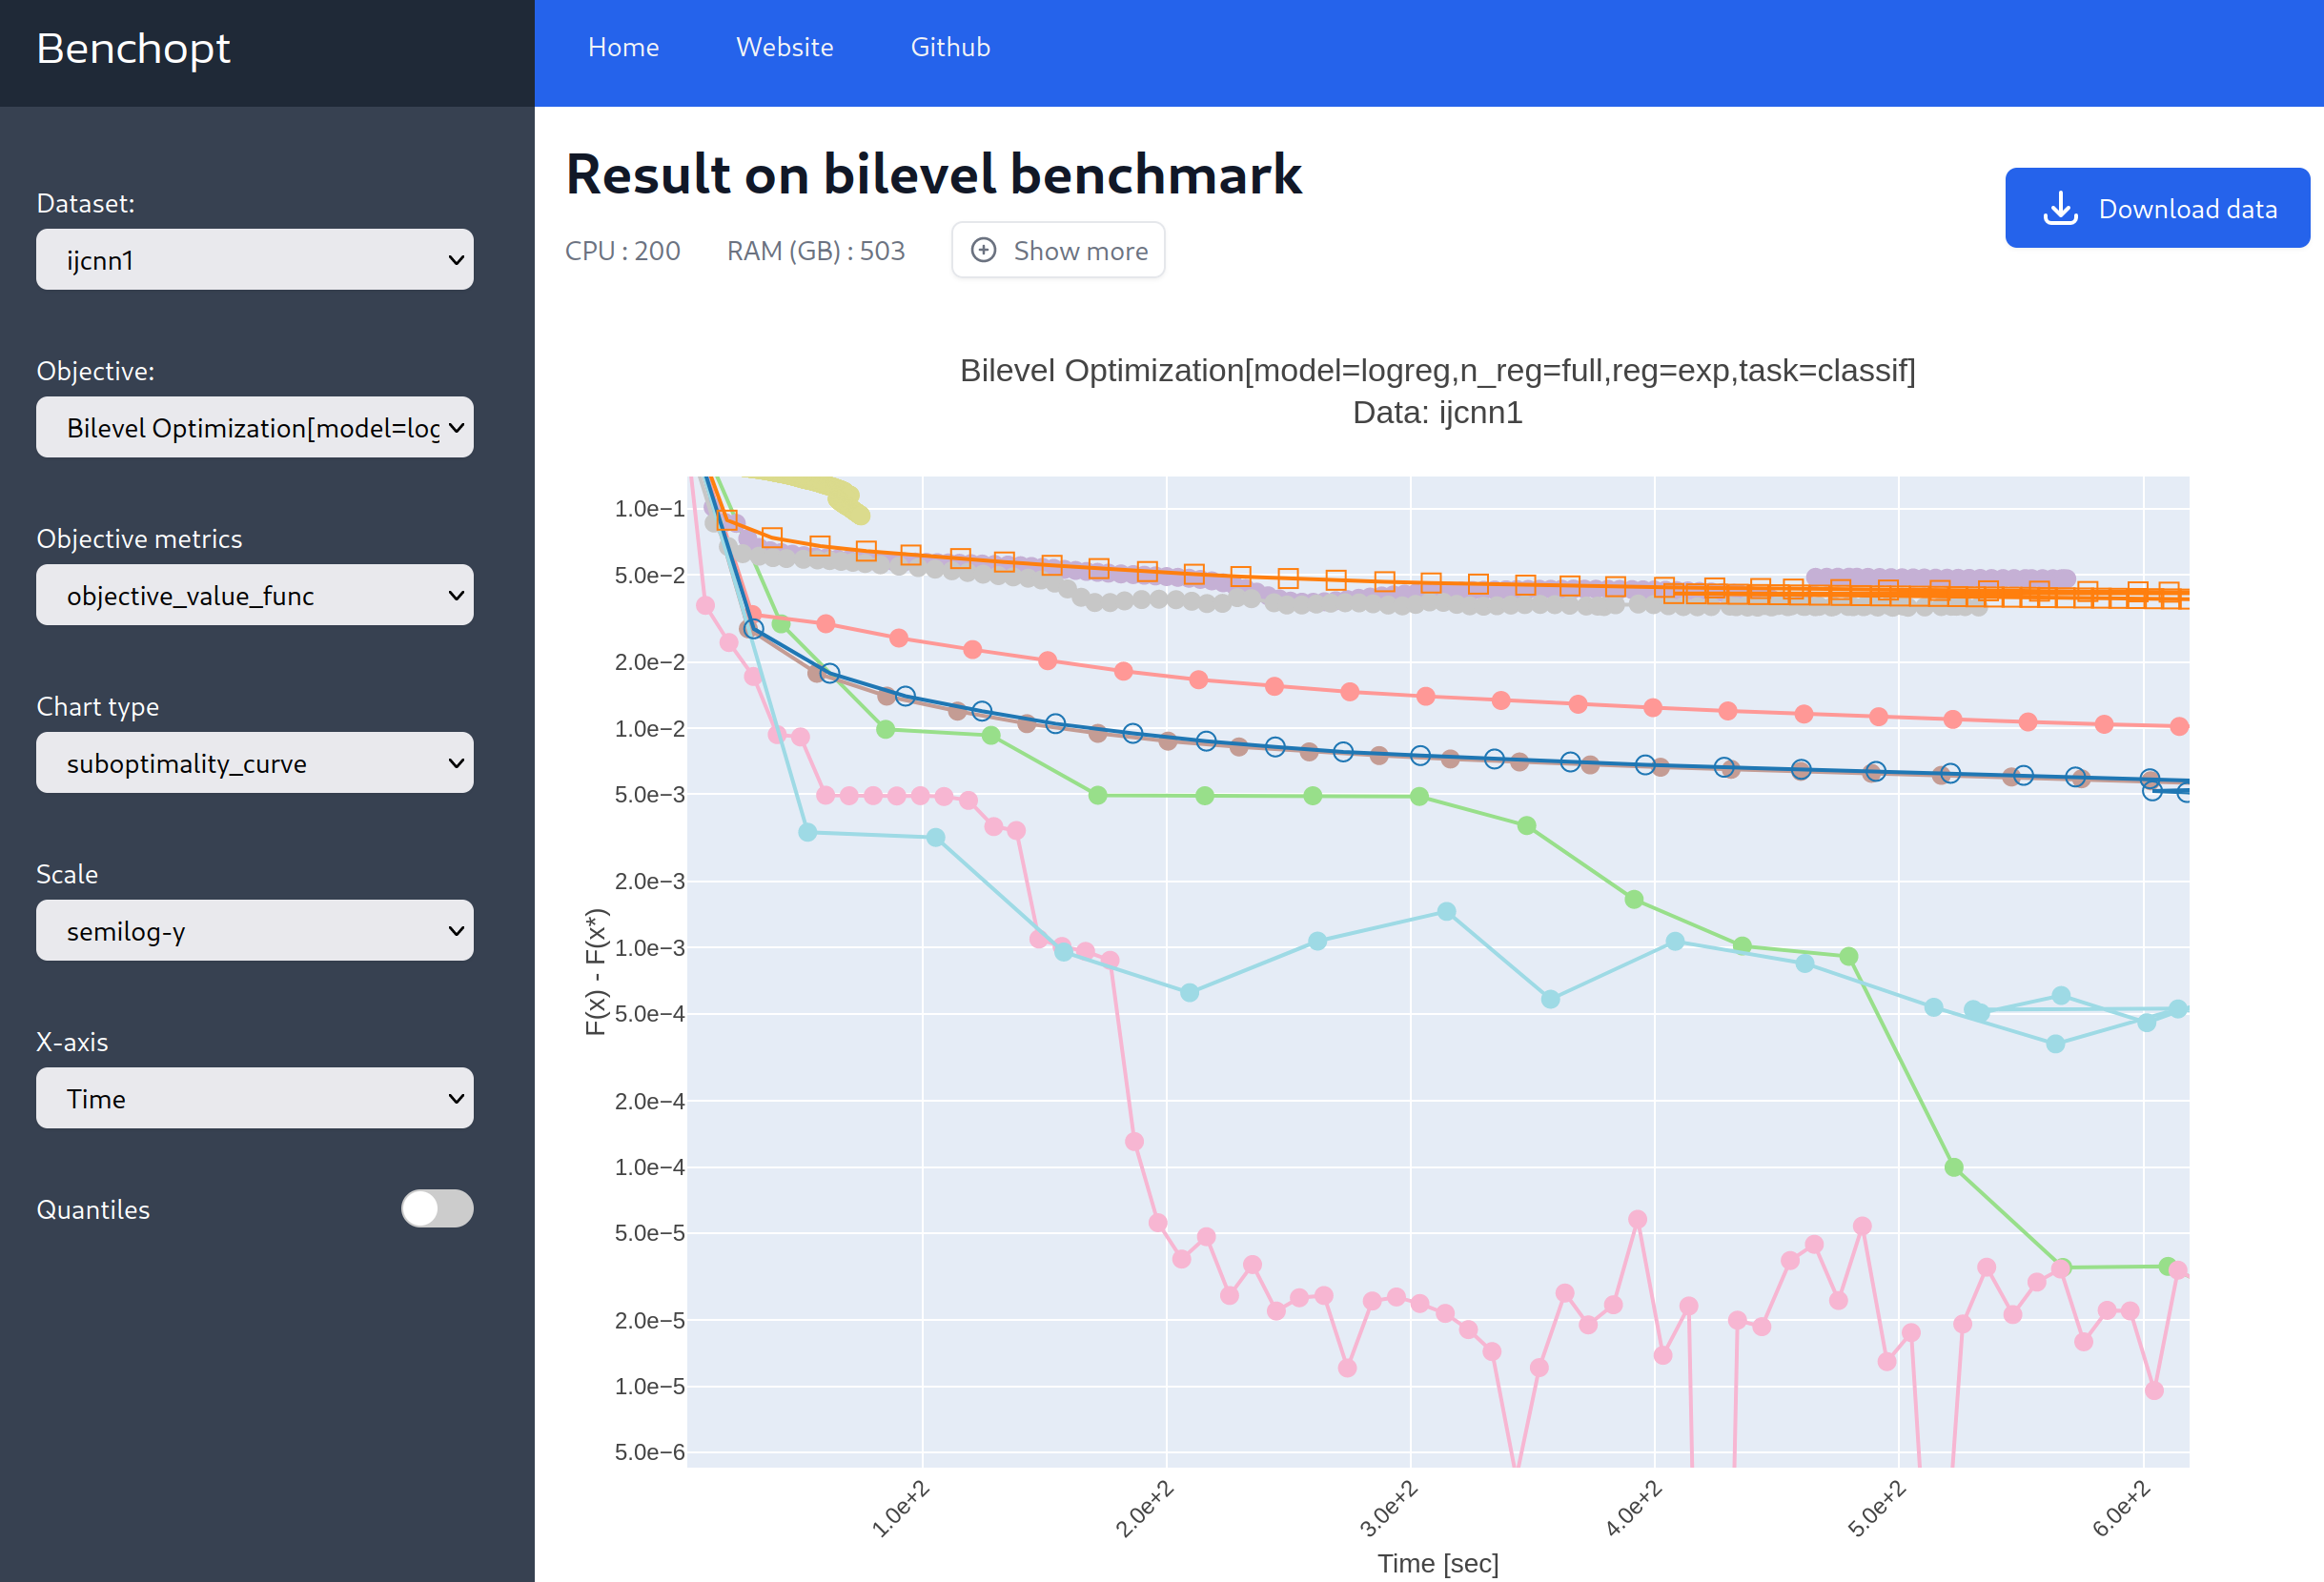
\includegraphics[width=.7\textwidth]{benchopt_bilevel}\\

% \hskip3ex
% 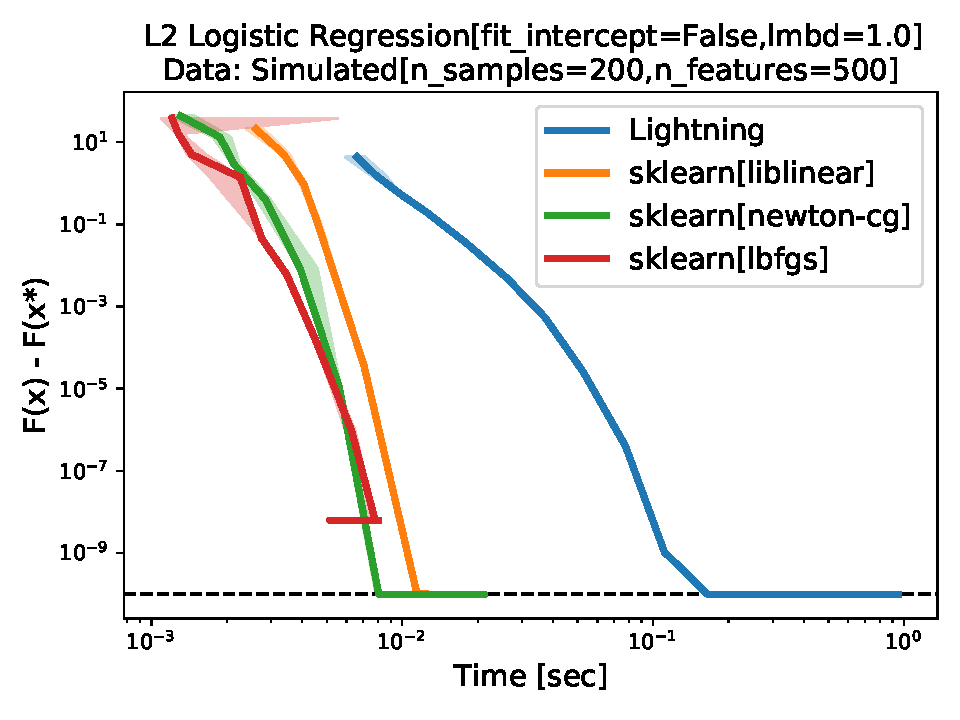
\includegraphics[width=.45\textwidth]{logreg_l2_1}

\end{frame}
%%%%%%%%%%%%%%%%%%%%%%%%%%%%%%%%%%%%%%%%%%%%%%%%%%%%%%%%%%%%%%%%%%%%%%%%%%%%%%%


%%%%%%%%%%%%%%%%%%%%%%%%%%%%%%%%%%%%%%%%%%%%%%%%%%%%%%%%%%%%%%%%%%%%%%%%%%%%%%%
\frame{
    \frametitle{Benchopt: principle}

    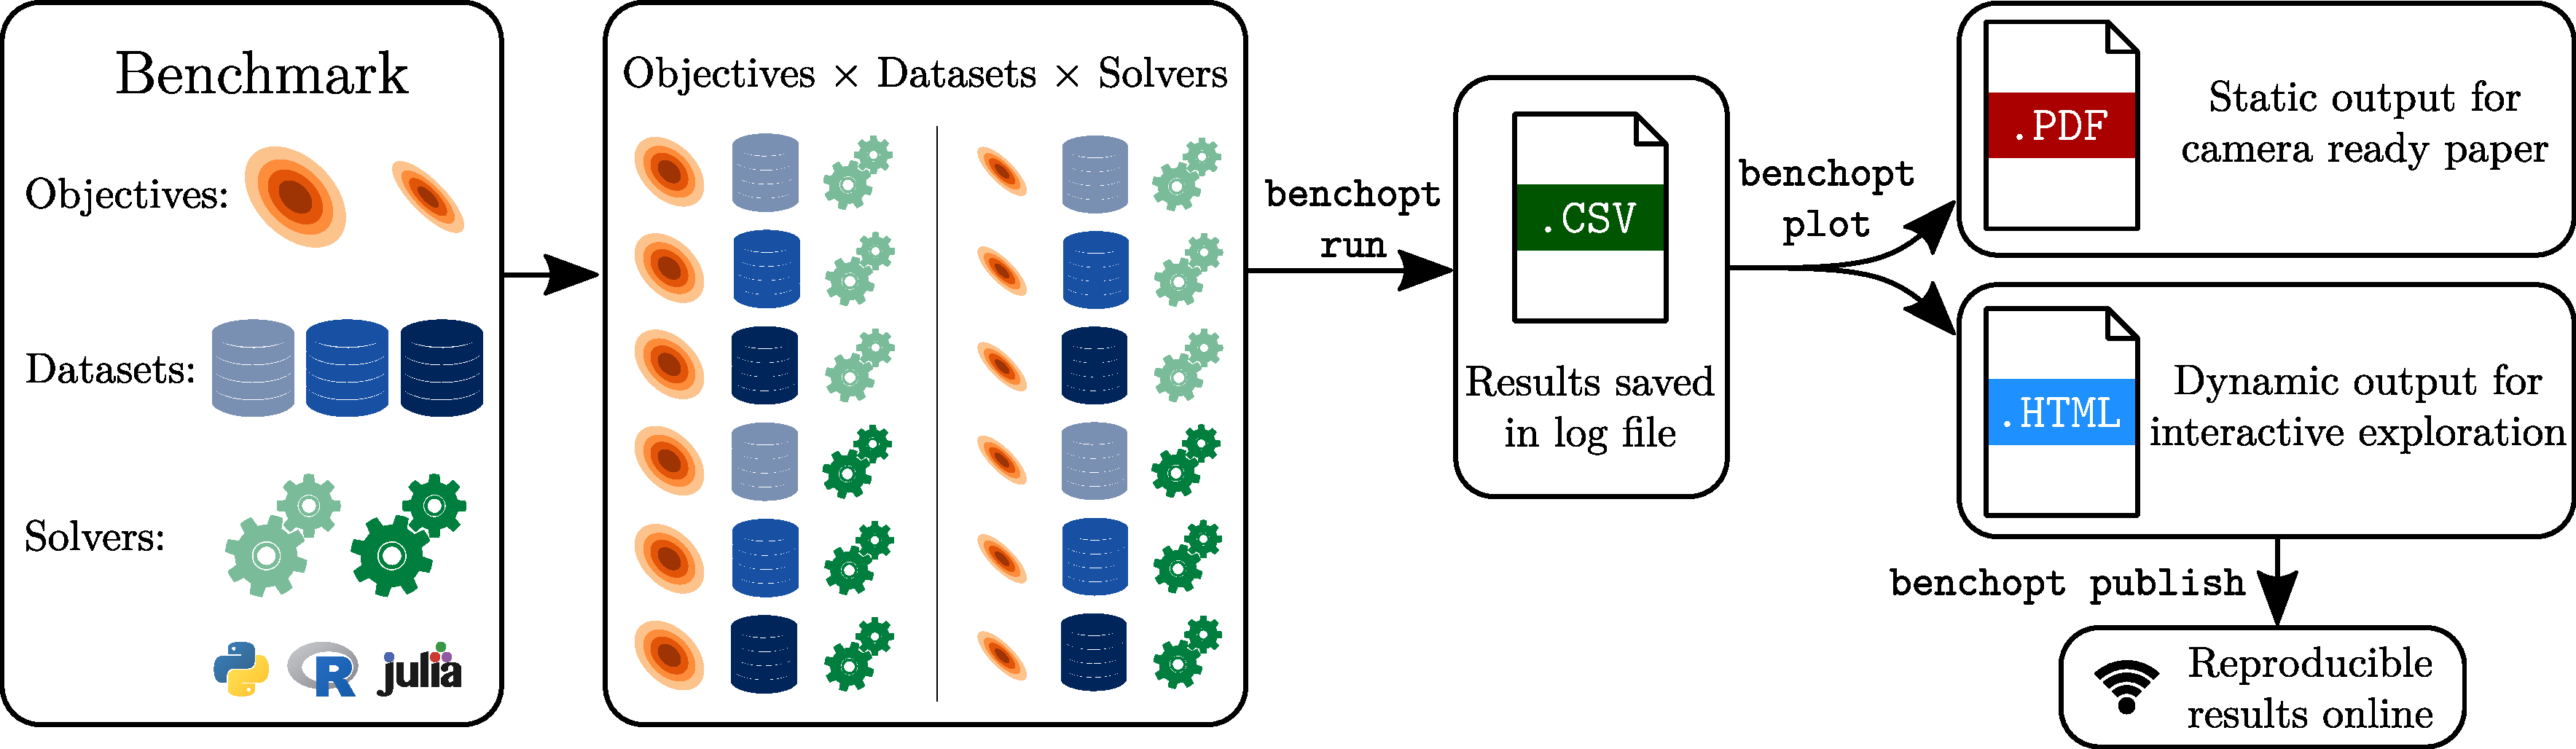
\includegraphics[width=\textwidth]{benchopt_schema_objectives_with_logos}

    \strongpoint{Each object can be parametrized so multiple scenario can be tested.}

    \vskip1.5em
    \textbf{Making tedious tasks easy:}\\[1em]
    \centering

    \myitem{} Sharing code
    \hskip3ex \myitem{} Adding methods
    \hskip3ex \myitem{} Exploring results\\[.5em]
    \myitem{} Varying hyperparameters
    \hskip3ex \myitem{} Running in Parallel
    \hskip3ex \myitem{} Caching\\[.5em]
    \hskip-4em\myitem{} \dots
}


%%%%%%%%%%%%%%%%%%%%%%%%%%%%%%%%%%%%%%%%%%%%%%%%%%%%%%%%%%%%%%%%%%%%%%%%%%%%%%%




\frame{
    \frametitle{Conclusion}

    \vskip2em
    \begin{itemize}\itemsep1em
        \item The propose framework allows to adapt many single-level algorithms to the bilevel setting.
        \item We get similar convergence rate in the bilevel setting,\\\emph{provided that we solve the inner problem fast enough}.
        \item \lstinline+Benchopt+ provides a benchmark to quickly test many ideas.
        \item One limitation is often the selection of learning rates.
    \end{itemize}

        \strongpoint{Toward adaptive algorithms for bilevel optimization?}


    \vspace{0pt plus 1 filll}
    Slides will be on my web page:\\[.5em]
    \hskip5em\includegraphics[height=.8em]{website} \url{tommoral.github.io}
    \hskip4em 
\includegraphics[height=.8em]{twitter} \href{https://twitter.com/tomamoral}{@tomamoral}

    }

    \appendix

    \section{Algorithm Unrolling}
    \parttitleframe[Differentiable inner problem solvers]{Shaban2019,Ablin2020,Malezieux2022}


    \frame{
        \frametitle{Differentiable unrolling of $\theta^t$}

        {\bf Idea:} \parbox[t]{.9\textwidth}{
            Compute $\frac{\partial \theta^t}{\partial \lambda}(\lambda) \approx \frac{\partial \theta^*}{\partial \lambda}(\lambda)$
            using automatic differentiation\\
            through an iterative algorithm.}\\[2em]

            \visible<2->{
                For the gradient descent algorithm:
                \[
                    \theta^{t+1} = \theta^{t} - \rho \frac{\partial G}{\partial \theta}(\lambda, \theta^t)
                \]
                The Jacobian reads,
                \[
                    \frac{\partial \theta^{t+1}}{\partial \lambda}(\lambda) = \Big(Id - \rho\frac{\partial^2 G}{\partial \theta^2}(\lambda, \theta^t) \Big)\frac{\partial \theta^t}{\partial \lambda}(\lambda) - \rho\frac{\partial^2 G}{\partial \theta\partial \lambda}(\lambda, \theta^t)
                \]
            }
            \visible<3->{
                \strongpoint{Under smoothness conditions, if $\theta^t$ converges to $\theta^*$,\\this converges toward $\frac{\partial \theta^*}{\partial \lambda}(\lambda)$}
            }
    }

    \frame{
        \frametitle{Analysis for min-min problems \rightcite{Ablin et al. 2020}}

        {\bf Context: } min-min problems where $F=G$\\
        \strongpoint{Here, $\frac{\partial F}{\partial \theta}(\lambda, \theta^*)= 0$}
        \vskip1em


        \visible<2->{
        We consider the $3$ gradient estimates:
        \begin{itemize}
            \item  $g_1 = \frac{\partial G}{\partial \lambda} (\lambda, \theta^t)$ \keypoint{Analysis}
            \item  $g_2 = \frac{\partial G}{\partial \lambda} (\lambda, \theta^t)
                + \frac{\partial G}{\partial \theta}(\lambda, \theta^t)\frac{\partial \theta^t}{\partial \lambda}
            $\keypoint{Automatic}
            \item  $g_3 = \frac{\partial G}{\partial \lambda}(\lambda, \theta^t)
            - \frac{\partial G}{\partial \theta}(\lambda, \theta^t)\frac{\partial^2G}{\partial \theta^2}^{-1}(\lambda, \theta^t) \frac{\partial^2 G}{\partial \theta\partial\lambda}(\lambda, \theta^t)
            $\keypoint{Implicit}
        \end{itemize}
        }
        \vskip2em
        \visible<3->{
            \begin{columns}
            \column{.55\textwidth}
            {\bf Convergence rates:} For G strongly convex in $\theta$,
            \begin{align*}
                |g^1_t(x) - g^*(x)| &= O\left(|\theta^t(\lambda)  - \theta^*(\lambda) |\right), \\
                |g^2_t(x) - g^*(x) | &= o\:\left(|\theta^t(\lambda)  - \theta^*(\lambda) |\right), \\
                |g^3_t(x) - g^*(x) | &= O\left(|\theta^t(\lambda)  - \theta^*(\lambda) |^2\right)  .
            \end{align*}
            \column{.4\textwidth}
            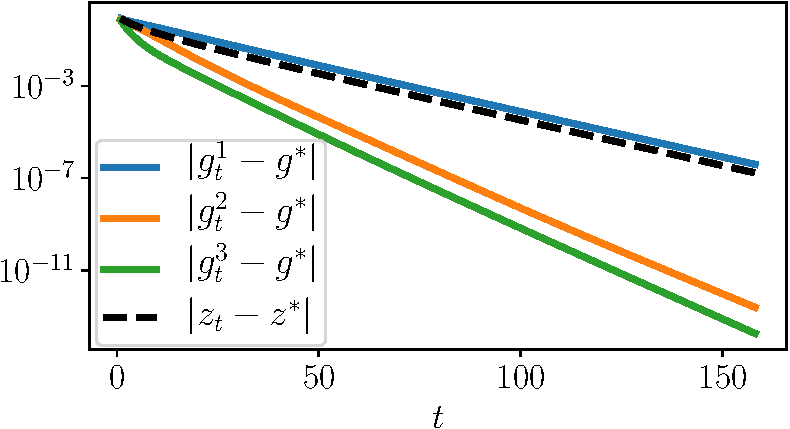
\includegraphics[width=\linewidth]{cvg_gradient}
            \end{columns}
        }
    }

    \frame{
        \frametitle{Analysis for non-smooth min-min problems \rightcite{Malezieux et al. 2022}}

        {\bf Context: } \parbox[t]{.8\textwidth}{dictionary learning, $F=G$ with an $\ell_1$-regularization for $\theta$.}

        \vskip2em
        {\bf Issue: } The implicit gradient quality mostly depends on the support identifiaction,
        \[
            {\Big(\frac{\partial\theta^*}{\partial D_l}\Big)}_{S^*} = -(D_{:, S^*}^\top D_{:, S^*})^{-1}(D_l {\theta^*}^\top + (D_l^\top \theta^* - y_l) Id_n)_{S^*} \enspace ,
        \]
        \vskip2em
        \strongpoint{Is the autodiff approach better than the analytic one?}
    }
    \frame{
        \frametitle{Analysis for non-smooth min-min problems \rightcite{Malezieux et al. 2022}}
        On the support, the function is smooth and we recover the same convergence.\\[1em]
        {\centering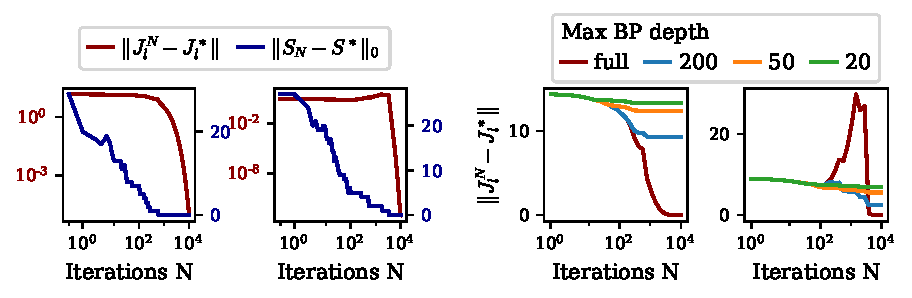
\includegraphics[trim={2.1em 2em 22em 1em}, clip, width=.8\textwidth]{conv_jac}\\}
    }

    \frame{
        \frametitle{Analysis for non-smooth min-min problems \rightcite{Malezieux et al. 2022}}
        Outside of the support, errors can accumulate and the gradient can blow up.\\[1em]
        {\centering 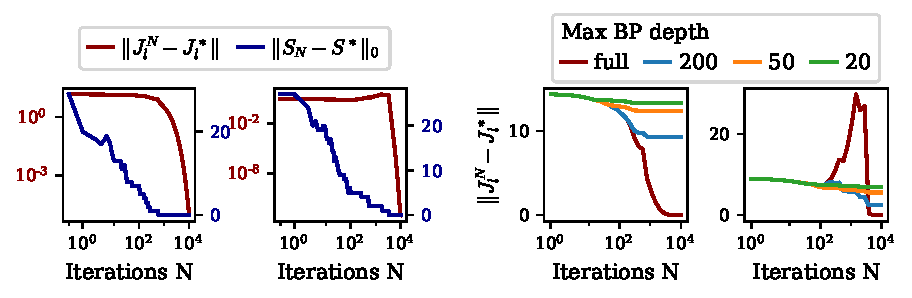
\includegraphics[trim={20.8em 2em .4em .5em}, clip, width=.8\textwidth]{conv_jac}\\
        }

    }



    \section{Hypergradient computation}
    \parttitleframe[]{Lorraine2020}

    \frame{
        \frametitle{Linear system approximation $v^*$}

        Solving the linear system for $v^*(\lambda^t)$,
        \begin{itemize}
            \item[$\bullet$] Core idea is to not inverse the hessian $\frac{\partial^2G}{\partial \theta^2}(\lambda^t, \theta^t)$,\\
            \keypoint{We are only interested in one direction.}
            \item[$\bullet$] Only rely on Hessian-vector product (Hvp).\\\keypoint{Can be computed efficiently}
        \end{itemize}

        \underline{\bf Proposed Methods:}\\[1em]
        \begin{columns}[T]
            \column{.4\linewidth}
            \myitem{} L-BFGS\\[1em]
            \myitem{} Jacobian-Free method
            \[
                \phantom{\sum_k}\frac{\partial^2G}{\partial \theta^2}(\lambda^t, \theta^t) \approx Id
            \]
            \column{.6\linewidth}
            \myitem{} Conjugate Gradient\\[1em]
            \myitem Neumann iterations
            \[
                \frac{\partial^2G}{\partial \theta^2}(\lambda^t, \theta^t)^{-1}\approx \sum_k (Id - \frac{\partial^2G}{\partial \theta^2}(\lambda^t, \theta^t))^k
            \]
        \end{columns}
        \vspace{0pt plus 1 filll}
        \rightcite{Pedregosa 2016, Lorraine et al. 2020, Luketina et al. 2016}


    }


\end{document}
